\chapter{\chapiiiname}
\label{chapter3}
 % insert abstract/summary here

\section{Introduction}
% Why does this chapters matter? What is the link to soft robotics and artificial skin/muscle?
% - Conductive particle elastomer composites are attractive for soft robotics because...
As discussed in Section \ref{sec:Piezoresistive Composites} conductive particle elastomer composites are desirable for soft sensor and actuator applications for a variety of reasons. However, it is crucial to understand the electromechanical behaviour of these composites if we wish to create complex control systems with such materials. Although conductive particle elastomer composites are a simple concept of dispersing particles throughout an elastomeric matrix, the electromechanical behaviour is not well understood on a macro or micro-scale. This section endeavours to understand the material behaviours of carbon black silicone rubber composites on a macro-scale to help create better inverse models so that the material can be used more accurately as a stress and/or strain sensor. 



\section{Material Imaging}
% This section will contain data gathered about the internal structure of the CBSR material. Including: Optical microscope, SEM, Raman spectroscopy, SAXS.
% Why is this section important? Ideally we would have an image of the percolated structure and how the particles move when deformed. However it is an arudous process to see nanometer scale structures using SEM or TEM and also run in-situ strain testing. Also the particles and agglomerates range from 50nm to ~5um in size, which means the largest particles can be seen with Raman and 50nm cannot be seen clearly by any method.
% What is the contribution towards research? Show some kind of patterning and agglomeration size??



\section{Stress and Resistance Relaxation For Carbon Nanoparticle Silicone Rubber Composite Large-Strain Sensors}
\label{sec:Stress and Resistance Relaxation}
\textit{From a conference paper presented at IDETC-MESA 2021}

Carbon nanoparticle-silicone elastomer composites are stretchable conductive materials with diverse applications such as, highly elastic strain sensors \cite{Lacasse2010,Spahr2017,Kim2018}, dielectric elastomer actuators \cite{Henke2018,Liu2009} and electromyography electrodes\cite{Carpi2010,Kim2018,Mouri2019}. Understanding the dynamic resistance relaxation characteristics of carbon black (CB) polydimethylsiloxane (PDMS) elastomer composites would improve performance in fields which require high efficiency of space, power and accuracy, such as the devices used in biomedical and aerospace fields. Unlike many common strain gauges, CB-PDMS composites can have strains of over 300\% without yielding\cite{Wang2010} depending on the type of PDMS and CB used and the method of fabrication. 


Some characteristics of CB-PDMS composites which make it suitable for strain sensors include that, the material is relatively inexpensive and readily available; non-toxic and is bio-compatible; and has a significant and readily measurable resistance change when stretched. Whereas, alternatives to CB nanoparticles, such as carbon nanotubes\cite{Maddipatla2017,Wang2013} and metallic particles\cite{Quinsaat2015,Racles2021}, have been seen to be more carcinogenic than the CB alternative\cite{Fukushima2018,Ferdous2020,Rausch2004}. The fabrication of the CB-PDMS composite requires a degree of optimisation to ensure that the carbon particles are adequately dispersed to ensure high conductivity and high yield strength of the material. More importantly the homogeneous dispersion of carbon black particles means better repeatability of experimental results and more accurate models for the eventual applications of CB-PDMS composites. A sufficiently comprehensive model of how the resistivity changes with strain has not yet been developed. A limitation of using this material as a strain sensor is the non-linearity of the material above a certain strain value, at which the composite's resistivity diverges towards a highly insulative value within the giga-ohms range. This non-linear behaviour of CB-PDMS can be used as a mechanically activated switching device\cite{Henke2018}. If modelled, this non-linearity could extend the range of strains that can be measured.

While previous work from our research group \cite{Giffney2017,Devaraj2018} has focused on the response to quasi-static and low speed behaviour, these materials show dynamic effects where resistance depends on the speed of stretching. The characterisation investigated for the CB-PDMS sensor involves understanding the relationship between the mechanical stress relaxation, electrical resistance relaxation and strain in time. A difference in time constants between the stress and resistance relaxations have been noted before in literature\cite{Kost1994,Wang2013,Maddipatla2017,Wang2004}, but never accurately modelled with the physical theory explained. The current limitations of predictability and repeatability of resistance relaxation hinders the accuracy of fitting models. An understanding of this resistance relaxation phenomena would mean an accurate model could be made to predict the relationship between stress, strain and resistance within a CB-PDMS composite. Finding this relationship model would also allow us to understand the limitations of using this composite in sensing applications and also the use of the material in dielectric elastomer actuators, whereby the material can be used simultaneously as an actuation excitation electrode and a strain sensor. The composite material can also be used in human motion measurement as a skin stretch sensor. Understanding these characteristics may give rise to new applications of the composites material, for example, if the resistive relaxation properties of the material were known, it could be used as a mechanically activated timing device. An oscillatory flexible dynamic circuit has been demonstrated when mimicking the motion of a caterpillar as shown by Henke et al.\cite{Henke2018}, where the resistance relaxation modelling is be useful for more accurate electrical circuit dynamics. The theory behind mechanical stress relaxation is widely known and has been modelled using a variety of mathematical models \cite{Fung1993} depending on the material modelled. The research discussed will focus primarily on only tensile stress of the specimen, and how it relates to the electrical resistive relaxation. 



\section*{BACKGROUND}
% TODO: add some bloatage here


\subsection*{The Composite}
The CB-PDMS composite was composed of carbon black powder(Vulcan XC 72R, average particle size: 50 nm, typical bulk density: 96 kg/m$^3$) and two part Pt cured PDMS(Smooth-On Dragon Skin 10 NV). This grade of PDMS was chosen due to the following characteristics \cite{SmoothOn2021}:
\begin{enumerate}
    \item Low elastic modulus, E, of 186 kPa
    \item Tensile strength, $\sigma_y$ of 2.75 MPa
    \item Low mixed viscosity, $\eta$, of 6,000 cps
\end{enumerate}
The volume resistivity of pure carbon black powder itself is between $10^{-1}$ and $10^2 \ \mathrm{\Omega cm}$ depending on how densely the particles are packed and the purity of the CB\cite{Spahr2017}. The ability of a carbon black matrix embedded within a highly insulative PDMS substrate to become conductive is determined mainly by the dispersion of the CB particles, and the tunneling that occurs between conductive CB and insulative PDMS bodies within the material volume\cite{Spahr2017,Wang2013}. The composite being created must be highly conductive without compromising the elastic modulus and yield strength of the material. From percolation theory observed in literature \cite{Spahr2017} there is a threshold volume percentage of CB required to ensure that conductivity is maintained with certainty throughout the composite volume within the linear volume resistivity region. The percolation threshold for our composite was is difficult to predict analytically due to the unknown configurations of aggregates and agglomerations formed by the CB within the composite material. Experimentally we found that a CB volume percentage of 7.5\% or greater meant the composite material had a resistivity of less than 3.5 $\mathrm{k\Omega cm}$ consistently with the fabrication method used.


\subsection*{The Mechanics}
It is known that PDMS composites are viscoelastic materials and clearly exhibit the three traits of a viscolelastic material\cite{Fung1993}: stress relaxation, strain creep and stress-strain hysteresis. Stress relaxation is effect observed when a step input of strain is applied to a material and there is a transient stress decay response which converges to a steady state value. A commonly used model for viscoelasticty is the generalized Maxwell body model of order $n$ shown in Fig. \ref{fig:Maxwell_general}.
\begin{figure}[H]
    \centering
    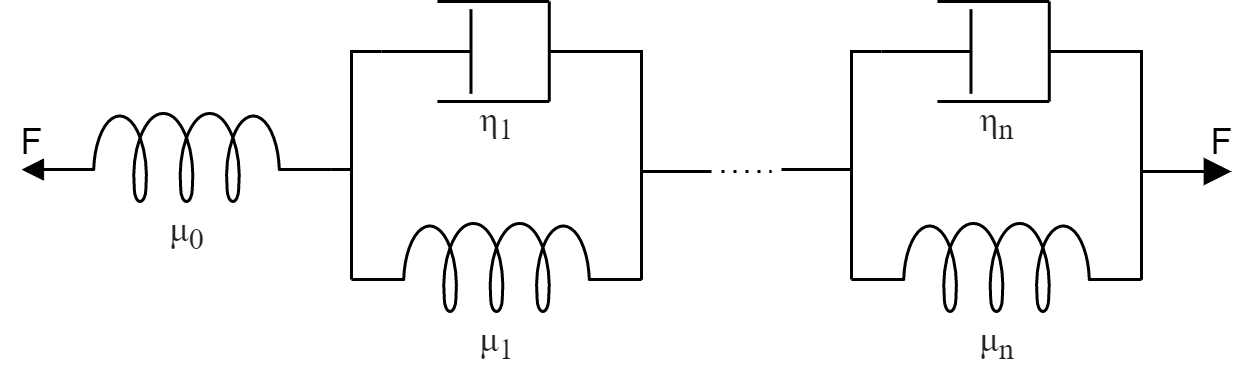
\includegraphics[width=8cm]{Figures/Generlised_Maxwell_body.png}
    \caption{MECHANICAL SPRING DASHPOT DIAGRAM OF THE GENERALIZED MAXWELL BODY MODEL ADAPTED FROM FUNG ET AL.\cite{Fung1993}}
    \label{fig:Maxwell_general}
\end{figure}
In Fig \ref{fig:Maxwell_general} $F$ is the force applied to the material and $\mu$ and $\eta$ values represent the spring and damping component constants, respectively. The stress relaxation function for this model is found in Eqn. \ref{eq:Maxwell_general}, for, $n$, serial repeating units. 
\begin{equation}
    G(t) = a_0 + \sum^n_{i=1} a_i e^{-t/\tau_i}
    \label{eq:Maxwell_general} 
\end{equation}
Where $a_0$, $a_i$ are the magnitudes of relaxation and $\tau_i$ are the relaxation decay time constant components. All of the constants $a_0$, $a_i$, and $\tau_i$ are functions of $\eta$ and $\mu$. 

% The relaxation function is made up of two functions, a reduced relaxation function, $K(t)$, and the elastic response function, $T_e(\varepsilon)$, such that,

% \begin{equation}
%     G(t) = K(t)T_e(\varepsilon)
%     \label{eq:stress_relaxation} 
% \end{equation}

We initially assume that there is a relationship between the stress relaxation and resistance relaxation of the material. However the generalized model can easily over-fit the data, if $n$ is too high, due to it's generality.



\section*{MATERIALS AND METHODS}
% TODO: add some bloatage here


\subsection*{Composite Fabrication}
The first step in fabrication was to mix the CB nano-powder with the silicone part A (the liquid PDMS elastomer) using a Kurabo KK-50S planetary mixer. A mixing function was used with specific rotational velocities and times for each axis, which was well suited towards de-aeration and viscous particle mixing. The material was then mixed with the silicone part B (the liquid PDMS elastomer cross-linker) using the same planetary mixing function to ensure adequate dispersion of the CB particles throughout the PDMS volume as well as de-aeration.
\begin{figure}[H]
    \centering
    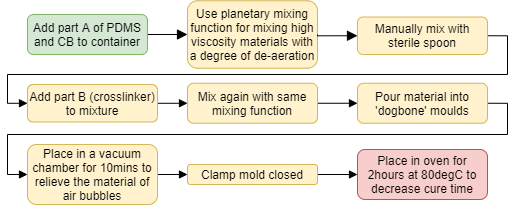
\includegraphics[width=9cm]{Figures/specimenPrepFlowDiagram (1).png}
    \caption{THE STEPS INVOLVED IN CREATING THE CB-PDMS COMPOSITE MATERIAL}
    \label{fig:CB-PDMS_flow_diagram}
\end{figure}
For the fabrication of the CB-PDMS specimens, a standard dog-bone shaped mould was developed for the mixed CB-PDMS to cure in, based on ASTM standard D412\cite{ASTM2020}. Before the mould was clamped shut the composite filled mould was immediately placed in a vacuum chamber for ten minutes to de-aerate the still liquid, curing CD-PDMS mixture. The specimen was placed in a controlled oven at a temperature of 80 $^{\circ}$C for a two hours to maintain the repeatability of the curing stage of the fabrication process. The temperature at which the silicone contributes towards the elastic modulus and yield strength of the material, with increasing curing temperatures giving increasing elastic moduli and decreasing yield strength values.


\subsection*{Measurement}
A custom test measurement device was made for measuring the desired characteristics of the CB-PDMS material, so that parameters driving the data collection could be easily altered. The strain, stress and resistivity of the specimen were measured in in parallel. The setup included the use of a 500 gram loadcell (HT sensor - TAL221) in combination with a linear actuator stage driven by a NEMA23 stepper motor and an source measurement unit (Keithley 2634B SMU). A custom electrode clamp mechanism was designed to fix the electrodes onto the test specimen during the straining of the specimen. This consists of two copper plates sandwiching the composite material at each end of the dogbone test specimen.
\begin{figure}[H]
    \centering
    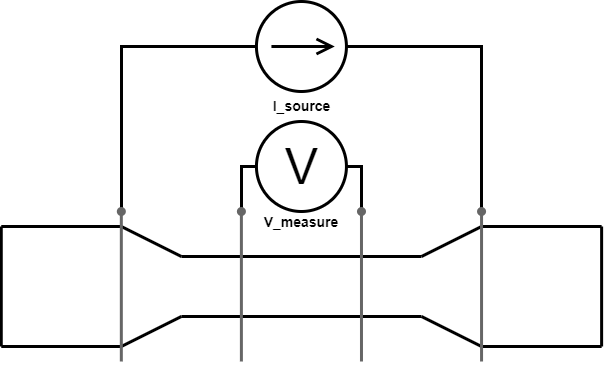
\includegraphics[width=5cm]{Figures/4wire_specimen.png}
    \caption{THE COMPOSITE DOGBONE TEST SPECIMEN PIERCED BY 4 PIN ELECTRODES. THE OUTER AND INNER ELECTRODES CONNECTED TO AN SMU CURRENT SOURCE AND VOLTMETER RESPECTIVELY}
    \label{fig:four_wire_dogbone}
\end{figure}
Two configurations of resistance measurement were tested, a two wire and a four wire method. The two wire measurement method used two electrodes which also clamped the test specimen at each end. It was observed that compressive strain applied to CB-PDMS composite will increase the resistivity of the specimen in a similar fashion to tensile stress. Only a compressive strain was applied to the material by the clamps such that the material would not slip during tensile testing and not deform giving erroneous resistance results. The Poisson's ratio of the material which was found experimentally to be 0.29 for both CB percentages. The two wire method used a controlled current source in parallel with a voltmeter attached to the same two electrodes to derive a resistance. The four wire method uses four pin electrodes as seen in Fig. \ref{fig:four_wire_dogbone}. The four wire method applies a constant current source through the outer electrodes and uses a voltmeter on the inner two electrode to determine the resistance and hence resistivity of the material. The four wire electrode configuration meant that the resistivity had a smaller signal to noise ration compared to a two wire alternative. 

Metallic pin electrodes were selected over copper clamp and conductive adhesive alternatives as they deformed the material the least, had a consistently low specimen-electrode contact resistance, and did not slip during test sequences. The inner pin electrodes were symmetric about the centre and placed 20 mm apart with the outer pin electrodes being 40mm apart as shown in Fig. \ref{fig:electromech-setup}.
\begin{figure}[H]
    \centering
    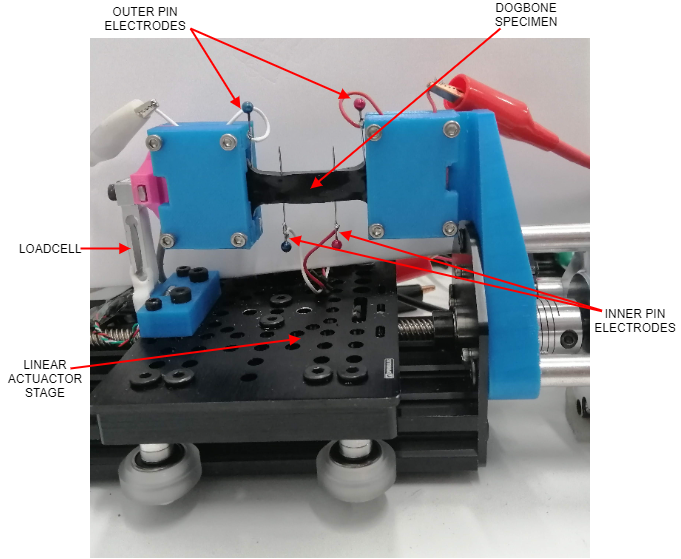
\includegraphics[width=9cm]{Figures/ELECTROMECH-SETUP.png}
    \caption{PHOTO OF TEST MEASUREMENT SETUP}
    \label{fig:electromech-setup}
\end{figure}
The measurements were completed using finite pulse trains of strain to ensure repeatability of the models were consistent across varying experimental parameters. If this material is used as a sensor the model fitted to the stress relaxation must hold over many consecutive tensile strain events. As these materials are intended as large strain sensors, the strains tested in this work was 10\%, 20\%, and 30\%. This strain percentage is higher than commonly used constantan strain gauges, which typically have a maximum strain of approximately $\pm 3$\%\cite{VishayPG2018}, with traditional metal alloy based strain gauges often having significant plastic deformation after less than $10^4$ cycles\cite{VishayPG2018} at 3\% strain.



\section*{RESULTS AND DISCUSSION}
% TODO: add some bloatage here 


\subsection*{Viscoelasticity}
All of the specimens fabricated indicated a degree of viscoelasticity shown by the hysteresis seen when loading and unloading the material with 30\% tensile strain in Fig. \ref{fig:loading-and-unloading-specimens}. The 0, 7.5, and 10 w.t.\% CB specimens have average elastic moduli, as measured in the loading phase, of 205.2 kPa\footnote{Different from the 186.2 kPa elastic modulus specified by the manufacturer due to the temperature accelerated curing method used}, 321.4 kPa, and 342.1 kPa, respectively. The hysteresis loop seen in the 10 w.t.\% CB sample has a larger hysteresis loop showing that there is increased viscous/damping compared with the other two specimens percentages of CB. The pure PDMS specimen had no discernible hysteresis from the data as shown in Fig. \ref{fig:loading-and-unloading-specimens}.  The difference in hysteresis and hence viscolelastic properties, across the specimens will lead to different stress relaxation properties across the three composite materials.
\begin{figure}[H]
    \centering
    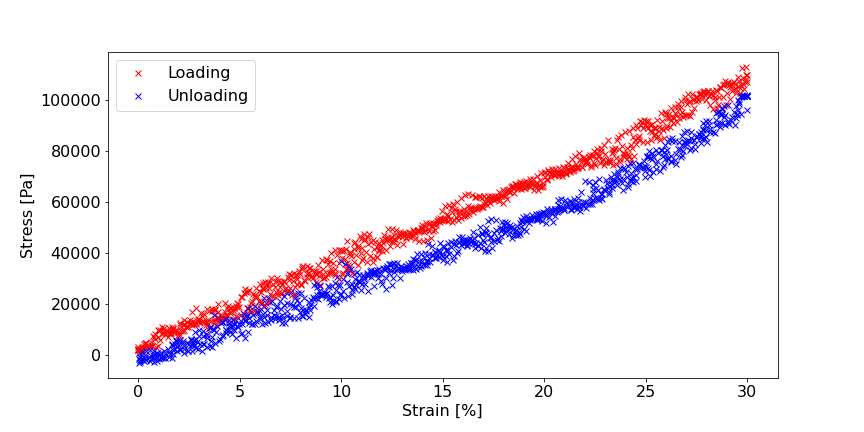
\includegraphics[width=10cm]{Figures/load_unload_1_10_E4pin_20mm_v9_0.3Strain.png}
    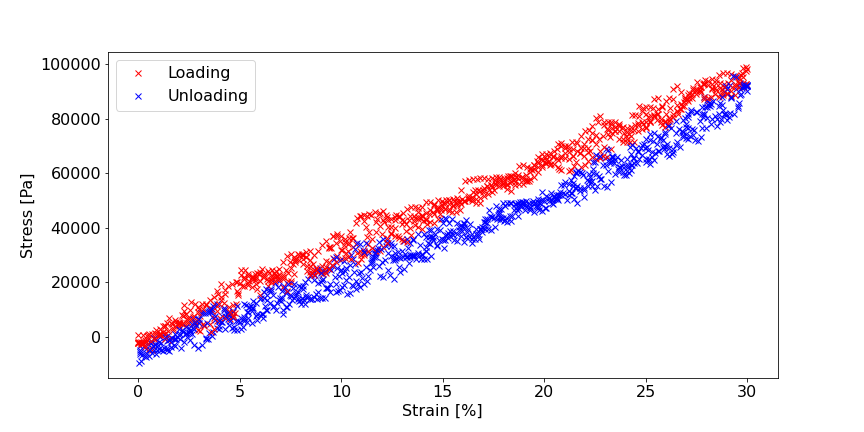
\includegraphics[width=10cm]{Figures/load_unload_2_7-5_E4pin_20mm_v10_0.3Strain.png}
    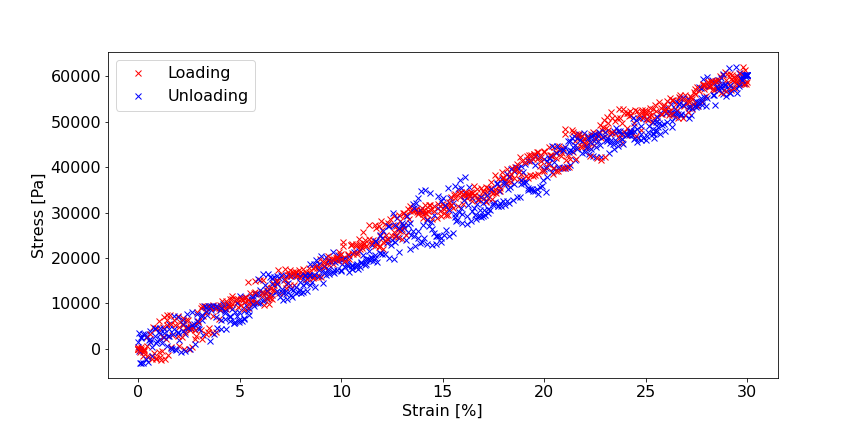
\includegraphics[width=10cm]{Figures/load_unload_1_CB0_v1_0.3Strain.png}
    \caption{THE LOADING AND UNLOADING OF 30\% STRAIN ON A COMPOSITE TEST SPECIMENS WITH CB WEIGHT PERCENTAGES FROM TOP TO BOTTOM OF 10\%, 7.5\%, AND 0\% WITH DATA COLLECTED OVER FIVE LOADING AND UNLOADING CYCLES}
    \label{fig:loading-and-unloading-specimens}
\end{figure}


\subsection*{Resistance Relaxation Model Fitting}
The initial model chosen to fit the stress and resistance relaxation data was the generalized Maxwell body model shown in Fig. \ref{eq:Maxwell_general} with n = 3 cascading elements using Eqn. \ref{eq:Maxwell_general_3elementS} to fit the model. Fitting the data using Levenberg–Marquardt non-linear least square algorithm over 30 data sets showed an instability with the algorithm using this model. When feeding the previously fitted stress relaxation model constants as initial conditions for the fitting of the next stress relaxation data set, the values of the constants diverged exhibiting signs of overfitting. This divergence of the model constants meant that they had a large standard deviation showing the model was changing significantly each iteration of fitting. Hence a more simple model using Eqn. \ref{eq:Maxwell_general} with n = 2 was used to fit the stress relaxation data to Eqn. \ref{eq:Maxwell_general_2elementS} with lower standard deviation of the model constants. Conversely when the resistance relaxation model analogous to stress relaxation model, shown in Eqn. \ref{eq:Maxwell_general_3elementR}, was fitted to the resistance relaxation data there was a stable fit with a better goodness of fit.

The decay time constants of the two models are different with the resistance having an longer overall decay which can clearly be seen in Fig. \ref{fig:diff_tau_res_stress}. Below in stress relaxation models $G_{1,2}(t)$, shown in Eqn. \ref{eq:Maxwell_general_3elementS} and \ref{eq:Maxwell_general_2elementS}, the constants $a_{0-3}$ and $\tau_{S1-S3}$ represent the components of magnitude and time decay of the stress relaxation, respectively.
\begin{equation}
    G_1(t) = a_0 + a_1e^{-t/\tau_{S1}} + a_2e^{-t/\tau_{S2}} + a_3e^{-t/\tau_{S3}}
     \label{eq:Maxwell_general_3elementS} 
\end{equation}
\begin{equation}
    G_2(t) = a_0 + a_1e^{-t/\tau_{S1}} + a_2e^{-t/\tau_{S2}}
     \label{eq:Maxwell_general_2elementS} 
\end{equation}
Analogously for the resistance relaxation function $H(t)$, the constants $b_{0-3}$ and $\tau_{R1-R3}$ represent the components of magnitude and time decay of the resistance relaxation, respectively. 
\begin{equation}
    H(t) = b_0 + b_1e^{-t/\tau_{R1}} + b_2e^{-t/\tau_{R2}} + b_3e^{t/\tau_{R3}}
     \label{eq:Maxwell_general_3elementR} 
\end{equation}
\begin{figure}[H]
    \centering
    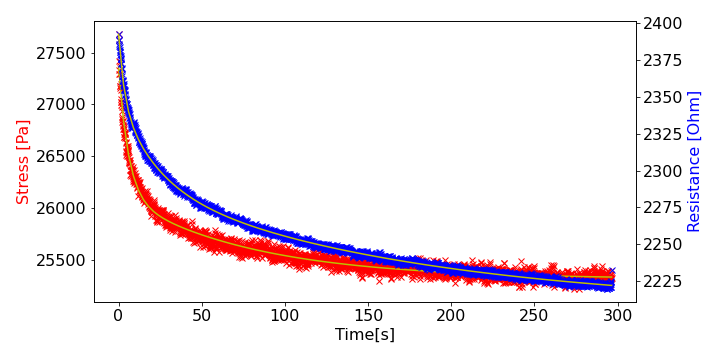
\includegraphics[width=9cm]{Figures/diff_time_const_Res_Stress_2_7-5_Epin_20mm_v3_pulse_6.png}
    \caption{COMPARING THE RELAXATION DECAY TIME CONSTANTS OF STRESS AND RESISTANCE FOR A 7.5 W.T.\% CB-PDMS COMPOSITE AFTER A 10\% STRAIN STEP INPUT AND FITTING GENERALIZED MAXWELL BODY MODELS TO EACH.}
    \label{fig:diff_tau_res_stress}
\end{figure}
The mean magnitude and decay time constants for the resistance and stress relaxations using 30 relaxation periods to fit the models to are given in table \ref{tab:generalised_model_constants}. The data gathered show that the stress relaxation time constant values decrease with an increasing carbon black percentage, indicating that all constants in Equations \ref{eq:Maxwell_general_3elementR} and \ref{eq:Maxwell_general_2elementS} are also functions of the carbon black percentage.

% \newpage
\begin{table}[h!]
\caption{FITTED CONSTANTS AND THEIR MEAN, $\mu$, STANDARD DEVIATION, $\sigma$, AND COEFFICIENT OF VARIATION, $CV$, VALUES FOR 0\%, 7.5\%, AND 10\% CB-PDMS COMPOSITE SPECIMENS USING EQUATION \ref{eq:Maxwell_general_2elementS}.}
\begin{center}
\label{tab:generalised_model_constants}
\begin{tabular}{c l l l}
\textbf{Stress Model} \\
0 \% CB Specimen \\
Constant & $\mu$ & $\sigma$ & $CV$ \\
\hline
$a_0$ & 20344.71 & 42.61 & 0.20\% \\
$a_1$ & 387.28 & 59.86 & 15.45\% \\
$a_2$ & 526.82 & 57.65 & 10.94\% \\
$\tau_{S1}$ & 72.08 & 23.46 & 32.54\% \\
$\tau_{S2}$ & 5.77 & 1.48 & 25.75\% \\
\hline
7.5 w.t.\% CB Specimen \\
Constant & $\mu$ & $\sigma$ & $CV$ \\
\hline
$a_0$ & 25363.89 & 33.62 & 0.13\% \\
$a_1$ & 802.32 & 43.59 & 5.43\% \\
$a_2$ & 1242.32 & 52.67 & 4.24\% \\
\end{tabular}
\end{center}
\end{table}
\begin{table}[h!]
\begin{center}
\label{tab:generalised_model_constants}
\begin{tabular}{c l l l}
$\tau_{S1}$ & 71.01 & 9.49 & 13.37\% \\
$\tau_{S2}$ & 5.79 & 0.65 & 11.32\% \\
\hline
10 w.t.\% CB Specimen \\
Constant & $\mu$ & $\sigma$ & $CV$ \\
\hline
$a_0$ & 32303.01 & 165.62 & 0.51\% \\
$a_1$ & 1071.38 & 54.32 & 5.07\% \\
$a_2$ & 1649.82 & 47.31 & 2.86\% \\
$\tau_{S1}$ & 84.07 & 10.55 & 12.54\% \\
$\tau_{S2}$ & 6.52 & 0.74 & 11.35\% \\
\hline
\end{tabular}
\end{center}
\end{table}
\begin{table}[H]
\caption{FITTED CONSTANTS AND THEIR MEAN, $\mu$, STANDARD DEVIATION, $\sigma$, AND COEFFICIENT OF VARIATION, $CV$, VALUES FOR 0\%, 7.5\%, AND 10\% CB-PDMS COMPOSITE SPECIMENS USING EQUATION \ref{eq:Maxwell_general_3elementR}.}
\begin{center}
\label{tab:generalised_model_constants}
\begin{tabular}{c l l l}
\textbf{Resistance Model} \\
7.5 w.t.\% CB Specimen \\
\hline
Constant & $\mu$ & $\sigma$ & $CV$ \\
\hline
$b_0$ & 2154.31 & 52.68 & 2.44\% \\
$b_1$ & 81.13 & 5.39 & 6.65\% \\
$b_2$ & 56.37 & 3.67 & 6.52\% \\
$b_3$ & 42.16 & 3.42 & 8.12\% \\
$\tau_{R1}$ & 181.10 & 33.57 & 18.54\% \\
$\tau_{R2}$ & 22.84 & 3.81 & 16.71\% \\
$\tau_{R3}$ & 3.46 & 0.56 & 16.35\% \\
\hline
10 w.t.\% CB Specimen \\
Constant & $\mu$ & $\sigma$ & $CV$ \\
\hline
$b_0$ & 1649.55 & 97.44 & 5.90\% \\
$b_1$ & 55.19 & 8.85 & 16.04\% \\
$b_2$ & 77.39 & 12.23 & 15.80\% \\
$b_3$ & 38.35 & 9.47 & 24.69\% \\
$\tau_{R1}$ & 169.63 & 61.72 & 36.38\% \\
$\tau_{R2}$ & 21.85 & 9.66 & 44.21\% \\
$\tau_{R3}$ & 3.02 & 1.59 & 52.72\% \\
\hline
\end{tabular}
\end{center}
\end{table}
Our aim was to prove the hypothesis that the stress relaxation time constant is different to that of the observed resistance relaxation and able to be modelled mathematically. The apparent difference in time constants and the fitting of the data to two different equations show that the stress relaxation is not linearly related to the resistance relaxation shown clearly in Fig. \ref{fig:diff_tau_res_stress}. To display the non-linear relationship between the stress and calculated resistance within the material they are plotted against each other over 30 sequential relaxation periods of 300s. The non-linear relationship between stress and resistance changes over time for each relaxation as shown in Fig. \ref{fig:res_vs_stress_30pulses}, where the data for the first relaxation is displayed in green and the last relaxation in blue.
\begin{figure}[H]
    \centering
    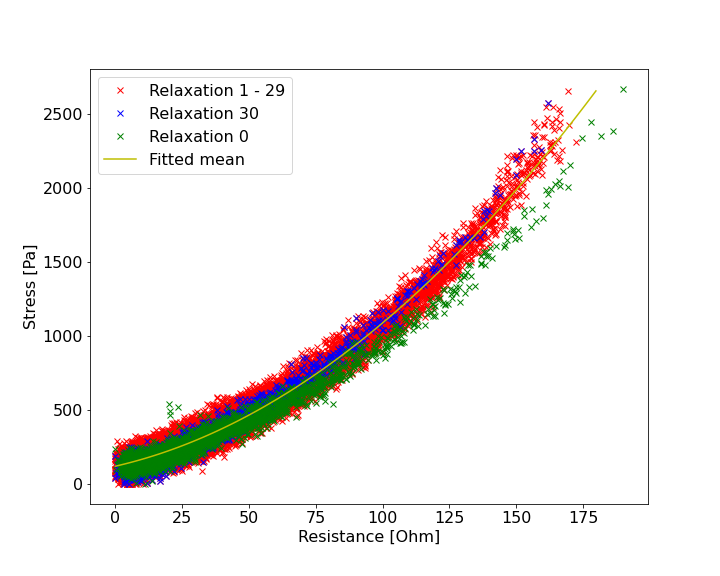
\includegraphics[width=10cm]{Figures/relax_res_stress_non_lin_rgby_MAF8_2_7-5_Epin_20mm_v3.png}
    \caption{COMPARING RESISTANCE AND STRESS RELAXATION DATA AGAINST EACH OTHER OCCURRING DURING 30 PULSES OF A 10\% STRAIN STEP INPUT FOR A 7.5 W.T.\% CB-PDMS COMPOSITE}
    \label{fig:res_vs_stress_30pulses}
\end{figure}
The stress-resistance relaxation data was fitted to a generic second order polynomial of the form, 
\begin{equation}
    \sigma(R) = aR^2+bR+c
    \label{eq:poly_res_stress}
\end{equation}
where $\sigma$ is stress, $R$ is the calculated resistance. When fit to the latter 15 cycles of a 30 cycle 10\% strain pulse train of stress relaxation data we get the constant values for $a$, $b$ and $c$.
\begin{table}[H]
\caption{FITTED CONSTANTS AND THEIR MEAN, $\mu$, STANDARD DEVIATION, $\sigma$, AND COEFFICIENT OF VARIATION, $CV$, VALUES FOR 7.5\%, AND 10\% CB-PDMS COMPOSITE SPECIMENS USING EQUATION \ref{eq:poly_res_stress}}
\begin{center}
\label{tab:generalised_model_constants}
\begin{tabular}{c l l l}
7.5 w.t.\% CB Specimen \\
Constant & $\mu$ & $\sigma$ & $CV$ \\
\hline
$a$ & 0.055 & 0.006 & 11.1\% \\
$b$ & 4.146 & 1.058 & 25.5\% \\
$c$ & 121.845 & 16.338 & 13.41\% \\
\hline
10 w.t.\% CB Specimen \\
Constant & $\mu$ & $\sigma$ & $CV$ \\
\hline
$a$ & 0.098 & 0.007 & 7.48\% \\
$b$ & 6.374 & 0.757 & 11.87\% \\
$c$ & 155.812 & 38.753 & 24.87\% \\
\hline
\end{tabular}
\end{center}
\end{table}


\subsection*{Strain Velocity Resistance Relationship}
A narrow peak in the apparent resistance has been observed in the collected data when changing from 10\% strain to a zero strain. This peak is not present in the stress plot, hence is a proposed characteristic of electrical behaviour only as a function of strain. In previous literature, the effects of the rate of change of strain on apparent resistance of the CB-PDMS material has not been modelled or shown. When the material has finished a tensile cycle of strain and is returning a zero strain state the a component of the resistance, $R_p$, can be modelled with a second order polynomial. When differentiated, this peak gives a linear function in a similar form of the linear strain curve seen in Fig. \ref{fig:poly2_r_strain}. Hence we form an equation which relates a component of resistance,
\begin{equation} 
%TODO: Double check this equation makes sense.
    \frac{dR_p}{dt} = E(\varepsilon)t + c
    \label{eq:dR_dt_strain}
\end{equation}
where $E$ is a function of strain, $\varepsilon(t)$, and c is an offset bias determined by the initial strain condition.
\begin{figure}[h!]
    \centering
    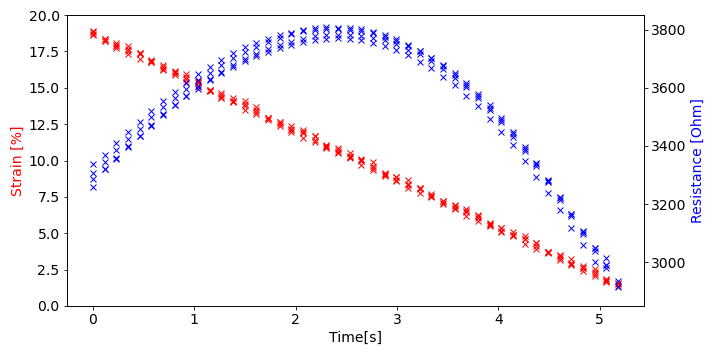
\includegraphics[width=8cm]{Figures/strain_velocity_res_80mms_2_7-5_E4pin_20mm_v11_0.2Strain_velocityprof.png}
    \caption{STRAIN VELOCITY RESISTANCE RELATIONSHIP SHOWING THE SPECIMEN IS RETURNING TO A 0\% TENSILE STRAIN STATE FROM 10\% AT A STRAIN RATE OF 80mm/s FOR FOUR TESTS FOR A 7.5\% CB-PDMS SPECIMEN}
    \label{fig:poly2_r_strain}
\end{figure}
To show the strain velocity resistance relationship, more strain pulse train tests of 20\% strain were completed. Using 20\% strain allowed us to see a sufficient number of data points to observe a trend. The pulses had four repetitions with a range of strain velocities, $\dot{\varepsilon}(t)$, of 40, 80, 120 and 160 $\mathrm{mms^{-1}}$. Using a 7.5 w.t.\% CB-PDMS specimen we obtain a relationship that agrees with the strain resistance component equation \ref{eq:dR_dt_strain}. As $\dot{\varepsilon}(t)$ increases through strain speeds so does the magnitude of the resistance peak (i.e. maximum height of the resistance peak - the previous steady state of value resistance) of 400, 510, 569, and 641 $\Omega$ for $\dot{\varepsilon}(t)$ of 40, 80, 120 and 160 $\mathrm{mms^{-1}}$  respectively. A new model is required which can accurately reproduce the additional decay time constant and small peak features seen in the resistance relaxation data, so that the resistance can inversely calculate the strain in the material. 

\subsection*{Repeatability}
The resistance relaxation model must be predictable over many strain cycles for use within many high stretch strain sensor application. If the resistance relaxation changes over time this needs is to be modelled. Each test sequence showed that there was a downward trend in the calculated magnitude of resistance for each pulse over time. This downward trend is hypothesized to be due to the accumulation of charge within material over time generated by current source, and was mitigated by using an alternating polarity measurement technique. The reversible current source helped to mitigate the capacitive effects seen, but a general downward trend in resistance was still observed as shown in Fig. \ref{fig:repeatability_pulse_trains}.  For every sufficiently long test sequence the material reaches a steady state, after a finite amount of time. The capacitance read across the inner pin electrodes of the material decreased with increasing strain as shown in Table \ref{tab:capacitance_v_strain}.
\begin{table}[H]
    \centering
    \caption{AVERAGE INNER ELECTRODE CAPACITANCES, $C_i$, MEASURED FOR VARIOUS STRAIN, $\varepsilon$, VALUES USING A 7.5 W.T.\% CB-PDMS COMPOSITE, MEASURED USING AN LCR METER AT 1kHz AND 10kHz \newline}
    \label{tab:capacitance_v_strain}
    \begin{tabular}{c||cccc}
        % \hline
        $\varepsilon [\%]$ & 0 & 10 & 20 & 30 \\
        \hline
        $C_i [pF]$ & 53 & 32 & 24 & 20 \\
        % \hline
    \end{tabular}
\end{table}
\begin{figure}[h!]
    \centering
    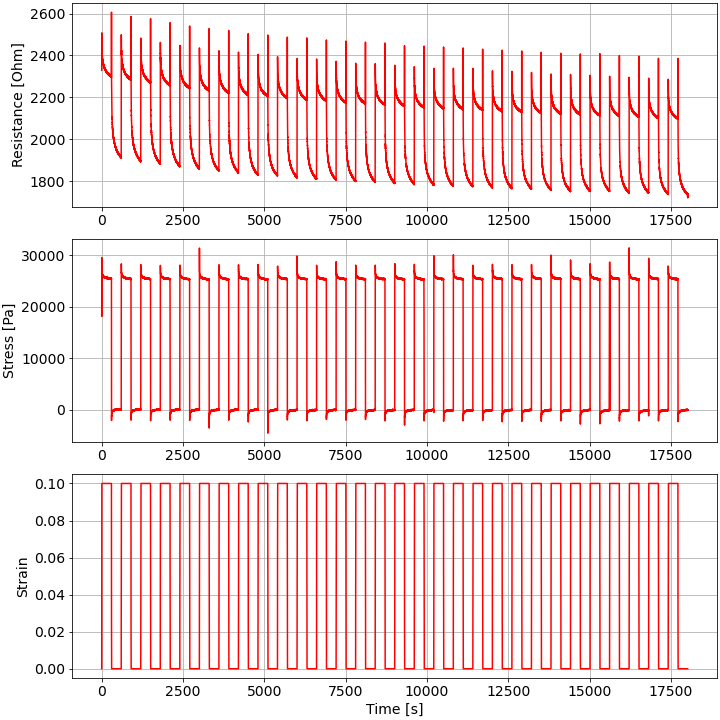
\includegraphics[width=9cm]{Figures/30_pulse_AC_2-7-5_Epin_20mm_v3.png}
    \caption{A TYPICAL TEST SEQUENCE OF A 30 PULSE STRAIN TRAIN RECORDING THE CALCULATED RESISTANCE AND STRESS OF A 7.5 W.T.\% CB COMPOSITE}
    \label{fig:repeatability_pulse_trains}
\end{figure}
The generalized Maxwell model has been applied to predict the stress relaxation of the CB-PDMS composite and analogously the resistive relaxation seen, which successfully explains a significant fraction of the resistance relaxation seen for a positive strain step input. However, a sudden peak of resistance when changing from +10\% strain to 0\% is not yet explained, and consideration of temperature and strain history\cite{Fung1993} will be useful to confirm the simple mathematical model given as Eqn. \ref{eq:dR_dt_strain}.

In this work, mixing has been performed using a planetary mixer. It has been shown in other works \cite{Xu2016,Spahr2017} that other mixing methods, such as using a sonication bath and the addition evaporateable solvents, can yield better particle dispersion. A higher degree of CB particle dispersion has also been shown to alter the viscoelastic creep properties \cite{Xu2016}, and is therefore likely to affect the time constant of resistance.


%%%%%%%%%%%%%%%%%%%%%%%%%%%%%%%%%%%%%%%%%%%%%%%%%%%%%%%%%%%%%%%%%%%%%%
\section*{CONCLUSIONS}
In order to improve the accuracy of dynamic strain measurements with CB-PDMS composites a stress and analogous resistance relaxation model was formed. The generalized Maxwell model, Eqn. \ref{eq:Maxwell_general_2elementS} was used to fit to the stress relaxation data for three specimen with CB weight percentages of 0, 7.5\% and 10\%. The CV of the stress relaxation magnitude constants $a_0-a_2$ were found to be consistently smaller than the CV of the stress relaxation decay time constants $\tau_{S1}$ and $\tau_{S2}$, with maximum CV values of 15.45\% and 32.54\% respectively. All of the stress relaxation model constants increased with increasing weight percentage of CB.

After modelling the stress relaxation, an analogous resistance relaxation model, Eqn. \ref{eq:Maxwell_general_3elementR} was formed and fitted to, displaying similar attributes to the stress relaxation model fit with all of the model constants increasing with increased w.t.\% CB. The CV of the analogous resistance relaxation magnitude constants $b_0-b_3$ were found to be consistently smaller than the CV of the stress relaxation decay time constants $\tau_{R1}-\tau_{R3}$, with maximum CV values of 16.04\% and 44.21\% respectively.

A model relating the resistance and stress relaxation has been developed using a second order polynomial with all of the constants $a$, $b$, and $c$ increasing with increased weight percentage of carbon black. With the models developed we have shown that the apparent resistance relaxation can be modelled, which will enable more accurate estimation of dynamic strain when these materials are applied as sensors. 
%%%%%%%%%%%%%%%%%% Paper finish.


\section{A Piece-wise Approach to Modelling Carbon Black Silicone Rubber Composites}
% Determining piece-wise all of the mathematical relationships seen between variables resistance, stress, strain, and time for CBSR test data.
% See CBSR behaviours document and flesh out with data!!
% Good paper: Experimental Investigation and Modeling of the Dynamic Resistance Response of Carbon Particle-Filled Polymers by Johannes Mersch et al
One method for understanding the transient behaviour of CPECs is to create a classification system and determine mathematical relationships that can be matched to these transient event. Mersch et al. have classified several shoulder events and the related deformation events, compressive, tensile, and bending. These transient peaks have been observed by several researchers using the similar CBSR materials, however there is no conclusive mathematical model relating these transient peaks to strain in time. This section aims to further classify these transient events and provide a mathematical relationship, for future use with model fitting methods.


\subsection{Rising Edge Step Response}


\subsection{Falling Edge Step Response}
As shown in Section \ref{sec:Stress and Resistance Relaxation} there has been a mathematical relationship observed between the falling edge of a strain input and the resultant resistance peak. Consequently a parameter fit study has been completed to determine how to predictably control the resistance peak through a controlled strain input. We can see a repeated property in Figure \ref{fig:poly2_r_strain} whereby the derivative of the resistance signal seems to be equal to the strain curve. 

To prove that there does exist a mathematical relationship between the two signals the relationship first each signal is given a generalised formula. The resistance signal is parabolic Equation \ref{eqn:gen_parabolic}. 
\begin{equation}
    R_p = A(t-H)^2 + K
    % A : concavity
    % H : horizontal shift
    % K : vertical shift
    \label{eqn:gen_parabolic}
\end{equation}
Where strain rate changes the vertical shift, K, time shift, H, and concavity, A, of the parabola. 

\subsection{Strain Rate}


\subsection{Saw Tooth Response}


\section{Characterising Hysteresis}
% see CBSR behavious doc